\documentclass[a4paper]{article}

\usepackage{tecnico_relatorio}


\usepackage[hypcap]{caption} % makes \ref point to top of figures and tables
\usepackage{rotating}
\usepackage{multirow}
\usepackage{geometry}
\usepackage{fancyvrb}

\begin{document}
	\trSetImage{img/tecnico_logo}{6cm} % Logotipo do Técnico
	\trSetSubject{Arquitecturas Avançadas de Computadores}
	\trSetType{Laboratório III - Paralelização e Aceleração de um Programa}

	
	\trSetBoxStyle{0.3}
	
	\trSetAuthorNr{3}
	
	\trSetAuthors
	{
		\begin{center}
			Gonçalo Ribeiro

			73294
		\end{center}
	}{
		\begin{center}
			Miguel Costa

			73359
		\end{center}
	}{
		\begin{center}
			Rafael Gonçalves

			73786
		\end{center}
	}
		
	\trSetProfessor{Prof. Leonel Sousa}
	
	\trMakeCover
	
	\tableofcontents
	\pagebreak
	
	\section{Introdução}
	
	O objectivo do presente trabalho laboratorial é a aceleração e paraleliazação de um algoritmo de \textit{smoothing}. Foi dada a possibilidade de realizar este projecto recorrendo a instruções vectoriais ou utilizando uma unidade de processamento gráfico (GPU), sendo que se escolheu utilizar instruções vectoriais suportadas pela arquitectura Intel IA32e (MMX, SSEx, AVX).
	
	O algoritmo de \textit{smoothing} consiste na obtenção de uma função aproximada, em que é filtrado todo o ruído resultante da amostragem do sinal. Na \autoref{fig:fun_smoothing} estão representados dois gráficos, em que o primeiro demostra o sinal com ruído e o segundo a função resultante após se aplicar a função de \textit{smoothing}.
	
		\begin{figure}[h]
			\centering
			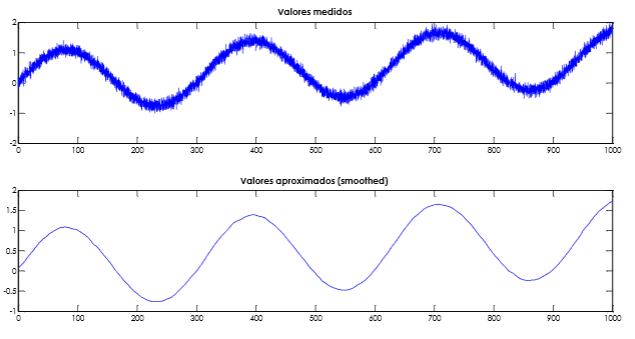
\includegraphics[width=1.\textwidth]{img/fun_smoothing}
			\caption{Resultado da aplicação de \textit{smoothing} a um sinal com ruído. }
			\label{fig:fun_smoothing}
		\end{figure}
		
	Para calcular o \textit{smoothing} foi fornecida a equação que permite calcular os valores aproximados $\hat{y}_1,\ ...\ , \hat{y}_{N-1}$, a partir da função original, com domínio $x_1,\ ...\ ,x_{N-1}$, e pontos (afectados de ruído) $y_1,\ ...\ , y_{N-1}$:
	
	\begin{equation}
		\hat{y}_i =  \frac{ \sum_{k=0}^{N-1} K_b (x_i, x_k ) y_k}{\sum_{k=0}^{N-1} K_b (x_i, x_k )} 
		\label{eq:smoothing_function}
	\end{equation}
	
	Onde
	
	\begin{equation}
		K_b (x_i,x_k)=exp\left(-\frac{(x-x_k)^2}{2b^2} \right)
		\label{eq:smoothing_kb}
	\end{equation}
	 	
	 	 
	Também é já fornecido no enunciado um algoritmo (Algoritmo 1) que ilustra um exemplo para calcular o resultado da função de \textit{smoothing}.
	
	
	\section{Aceleração e Paralelização}
	
	Para realizar a aceleração do programa foram adoptadas várias estratégias: usando instruções de processamento vectorial de 128 bits e usando instruções de processamento vectorial de 128 bits com \textit{unrolling} do ciclo de computação em 2, 3, 4 e 8 cálculos por ciclo.
	
	A primeira tarefa a executar é então alocar a memória necessária para os dados e para os resultados. Para tal usou-se uma função já fornecida pelo professor (\texttt{aligned\_malloc()}) que permite alocar um tamanho desejado de memória, com a particularidade de que é garantido que esta memória está alinhada na memória. Tal não é garantido pela função \texttt{malloc()} e para o uso das instruções vectoriais é imprescindível que os dados a processar estejam alinhados.
	
	De seguida são corridas as funções em teste. Os resultados de todas as soluções com instruções vectoriais são comparadas com uma função escrita directamente com base no Algoritmo 1 do enunciado, a que se chamou \texttt{normal\_smoothing()}:
	
	\begin{verbatim}
void normal_smoothing(float *x, float *y, float *res, int len) {
    int i,j;
    float sumA, sumB, factor;
    
    for(i=0; i<len; i++){
        sumA = sumB = 0;
        for(j=0; j<len; j++){
            factor = exp((-(x[i]-x[j])*(x[i]-x[j]))/(2*_SMOOTH*_SMOOTH));
            sumA += factor*y[j];
            sumB += factor;
        }
        res[i] = sumA/sumB;
    }
}
	\end{verbatim}
	
	
	Antes de se medir qualquer tempo, o algoritmo em análise é corrido uma vez, de modo a tentar que as instruções e dados estejam em \textit{cache}. Isto é feito tanto para as soluções com instruções vectoriais como para a função \texttt{normal\_smoothing()}.
		
	Após se obterem os diversos valores temporais, é liberta a memória anteriormente alocada e são verificados os resultados do \textit{smoothing} obtidos de modo a comprovar se se chegou ao resultado desejado: remover o ruído do sinal original.
	
	\subsection{\texttt{smoothing\_simple()}}
	
	Esta função implementa o algoritmo de \textit{smoothing} recorrendo a instruções vectoriais. O ciclo interno é paralelizado visto que cada operação é feita sobre 4 ou 8 dados em simultâneo (conforme se esteja a usar a versão de 128 bits ou a de 256).
	
	Uma optimização que foi feita foi fazer uma única divisão por cada chamada da função: embora a função de \textit{smoothing} contenha uma divisão que é feita $i \times j$ vezes o divisor é constante, pelo que a optimização utilizada consiste em calcular o inverso do divisor uma única vez e a partir desse momento usar sempre multiplicações. Isto resulta numa optimização porque segundo Intrinsics Guide da Intel as divisões com instruções vectoriais demoram mais ciclos do que as multiplicações.
	
	Como exemplo apresenta-se a função \texttt{sse128\_smoothing\_simple()}, que consiste na implementação da \texttt{smoothing\_simple()} para instruções vectoriais de 128 bits. Para alocar o vector \texttt{aux} usou-se a \texttt{aligned\_malloc()} visto que a função \texttt{\_mm\_store\_ps()} escreve para uma posição alinhada de memória.
	
	\begin{verbatim}
void sse128_smoothing_simple(float *x, float *y, float *res, int len) {
    float *xi, *xj, *yj;
    float *aux = (float*) aligned_malloc(4*sizeof(float));
    float sumAtot, sumBtot;

    __m128 sumA, sumB;
    __m128 divisor = _mm_div_ps(_mm_set_ps1(1.0), _mm_set_ps1(2*_SMOOTH*_SMOOTH));
    __m128 exponential;
    __m128 cache;

    for(xi=x; xi < x+len; xi++, res++)
    {
        sumA = sumB = _mm_setzero_ps();

        for(xj=x, yj=y; xj < x+len; xj+=4, yj+=4)
        {
            // e^[(-(xi-xj)^2) / (2*smoothing^2)]
            cache = _mm_sub_ps(_mm_load_ps1(xi), _mm_load_ps(xj));
            
            exponential = _mm_exp_ps(
                    _mm_mul_ps(
                        _mm_sub_ps(_mm_setzero_ps(),
                            _mm_mul_ps(
                                cache,
                                cache
                                )), divisor));

            sumB = _mm_add_ps(sumB, exponential);
            sumA = _mm_add_ps(sumA, _mm_mul_ps(_mm_load_ps(yj), exponential));
        }

        // horizontaly add sumA and sumB
        _mm_store_ps(aux, _mm_hadd_ps(_mm_hadd_ps(sumA, sumB), _mm_setzero_ps()));

        sumAtot = aux[0];
        sumBtot = aux[1];

        *res = sumAtot/sumBtot;
    }

    aligned_free(aux);
}
	\end{verbatim}		

	
	\subsection{\texttt{smoothing\_unroll*()}}
	
	Para tentar acelerar ainda mais o algoritmo desenvolvido, foi testado a execução de \textit{unrolling} no ciclo de computação. Nesse sentido foram testados 4 casos de \textit{unrolling}: 2, 3, 4 e 8 instruções por ciclo, sendo que se pode concluir que o aumento de instruções por ciclo tende a aumentar ligeiramente o speedup obtido.
	
	
	\section{Testes} 
		
	Para testar a aceleração do nosso programa foram comparados os tempos de execução do algoritmo 1 com os programas desenvolvidos pelo grupo para acelerar o algoritmo 1. A tabela seguinta demonstra o tempo de execução do algoritmo 1 (Tempo Original) e os \textit{speedups} encontrados para diferentes tamanhos de vectores (entre 16 e 16384 \textit{floats}) para as várias estratégias desenvolvidas:
	

	\begin{table}
	\caption{Resultados para extensões multimédia de 128 bits}
	\label{tab:results_128}
	\begin{Verbatim}[fontsize=\small,xleftmargin=-5mm]
=============================================================================================
   COMPUTING SMOOTHING SPEEDUP for SSE-128
=============================================================================================
| Vector |   Original |   speedup   |   speedup   |   speedup   |   speedup   |   speedup   |
| Length |  Time [us] |    simple   | unrolling 2 | unrolling 3 | unrolling 4 | unrolling 8 |
+--------+------------+-------------+-------------+-------------+-------------+-------------+
|     16 |        4.6 |    0.884615 |    0.958333 |    0.410714 |    0.920000 |    0.171642 |
|     32 |       61.2 |    3.090909 |    3.600000 |    4.935484 |    5.563636 |    4.309859 |
|     64 |      237.4 |    2.799528 |    3.618902 |    2.580435 |    3.450581 |    3.440580 |
|    128 |      929.4 |    3.812141 |   10.707373 |   10.146288 |    4.732179 |    4.302778 |
|    256 |     2006.2 |    4.965842 |    5.876391 |    5.591416 |    6.393244 |    5.499452 |
|    512 |     4689.4 |    3.082698 |    3.663021 |    3.795241 |    3.982167 |    3.940010 |
|   1024 |    21119.0 |    2.736969 |    3.145236 |    3.231478 |    3.362470 |    3.361292 |
|   2048 |    93695.2 |    2.919054 |    3.363386 |    3.491712 |    3.595585 |    3.606880 |
|   4096 |   408000.6 |    3.171430 |    3.693677 |    3.836525 |    3.947367 |    3.982164 |
|   8192 |  1634784.8 |    3.165204 |    3.724790 |    3.882026 |    3.964539 |    4.029549 |
|  16384 |  6482300.2 |    3.153480 |    3.720566 |    3.879947 |    3.960604 |    4.033608 |
|  32768 | 25781057.0 |    3.144238 |    3.711833 |    3.877029 |    3.953504 |    4.032080 |
+--------+------------+-------------+-------------+-------------+-------------+-------------+
	\end{Verbatim}
	\end{table}


	
	\section{Demonstração \textit{vs.} Desenvolvido}
	
	 Aquando a demonstração, os resultados de speedup obtidos eram muito inferiores ao esperado (estando-se a obter valores de speedup próximos de 1). Contudo, após uma análise mais detalhada sobre o funcionamento de instruções vectoriais, verificou-se que, apesar da não se estar a usar a porção de código correspondente ao uso de instruções de processamento vectorial para 256 bits, o facto de existir esta porção de código fazia com que o compilador agendasse mudanças de modo entre o processamento de 128 bits e o de 256 bits, o que atrasava imenso a execução do programa. Como tal separam-se estas duas componentes de processamento em dois programas distintos. Esta simples mudança fez com que, ao usar as instruções de processamento de 128 bits, se conseguisse atingir resultados de speedup próximos do esperado.
	   
	
	
	
	\section{Conclusão}

\end{document}
